%!TEX root = ../template.tex
%%%%%%%%%%%%%%%%%%%%%%%%%%%%%%%%%%%%%%%%%%%%%%%%%%%%%%%%%%%%%%%%%%%%
%% chapter4.tex
%% NOVA thesis document file
%%
%% Chapter with lots of dummy text
%%%%%%%%%%%%%%%%%%%%%%%%%%%%%%%%%%%%%%%%%%%%%%%%%%%%%%%%%%%%%%%%%%%%

\typeout{NT FILE chapter4.tex}%


\chapter{Scan, Point Cloud Processing, and CAD Model}
\label{cha:digi}


\section{Scanning Process of the Compressor Blade}
\label{sec:scan}

To generate an accurate digital model of the compressor blade, it was crucial to capture a complete and detailed point cloud of its geometry. Given the complex shape and critical role of the blade, a structured approach was followed to ensure precision in data acquisition and processing. The scanning process was designed to encompass all necessary surfaces while minimizing errors and distortions.

The first step in the scanning process involved attaching positioning targets to a fixed table. A technician from the Dimensional Inspection department at \gls{TAP} carried out the scan using the Creaform HandyScan, a handheld 3D scanner. As represented in Figure~, the targets placed on the table provided reference points that enhanced accuracy and enabled precise alignment of the scans. By positioning the blade in different orientations, it was possible to capture data from multiple angles, ensuring complete surface coverage. The VXelements software utilized these positioning targets to align the scans more precisely.

For this particular case, scanning was performed with the blade placed in two different positions. This ensured that all necessary surfaces were captured. After obtaining the individual scans, the merging process was conducted using the best-fit alignment method. This method, which employs an iterative closest point algorithm, minimizes the squared distances between overlapping scan points, thereby achieving a seamless integration of the different scans into a single mesh.

During the scanning process, the reflective nature of the blade’s surface further complicated the scanning process, causing inconsistencies in data capture. In some cases, fine particles such as talcum powder can be applied to reduce reflections and improve scan quality. For the sixth stage blade scan an error also occurred in the scanning process that resulted in missing data from a non-functional surface of the blade. This missing data is represented in Figure~\ref{fig:zonadanf} with a blue mark. This issue was addressed within VXelements by performing mesh processing to refine and correct the scanned model.

\begin{figure}[H]
    \centering
    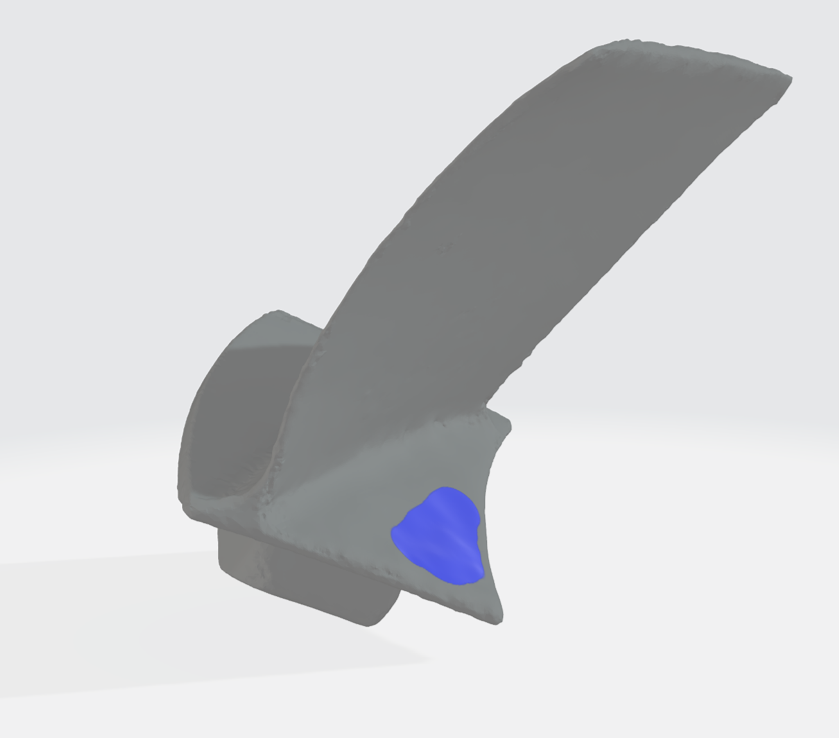
\includegraphics[width=0.5\textwidth]{zonadanf}
    \caption{Missing data in Scan}
    \label{fig:zonadanf}
\end{figure}

VXelements was utilized to remove unwanted points captured from the surrounding environment to enhance the final mesh quality. Furthermore, specific mesh processing tools were applied to address minor irregularities and fill non-critical gaps. However, it is important to note that the wide and narrow regions of the blade did not require scanning, as their impact on the overall accuracy was minimal. This aspect will be further elaborated in the Blade CAD Model Accuracy section.

In summary, the scanning process for the compressor blade involved multiple viewpoints, best-fit merging, and mesh refinement to achieve a high-quality digital representation. Despite minor challenges, the final scans provided a reliable foundation for further CAD modeling and analysis. Figure~\ref{fig:scan1} presents the point cloud obtained from the scanning process of the Sixth Stage blade.

\begin{figure}[H]
    \centering
    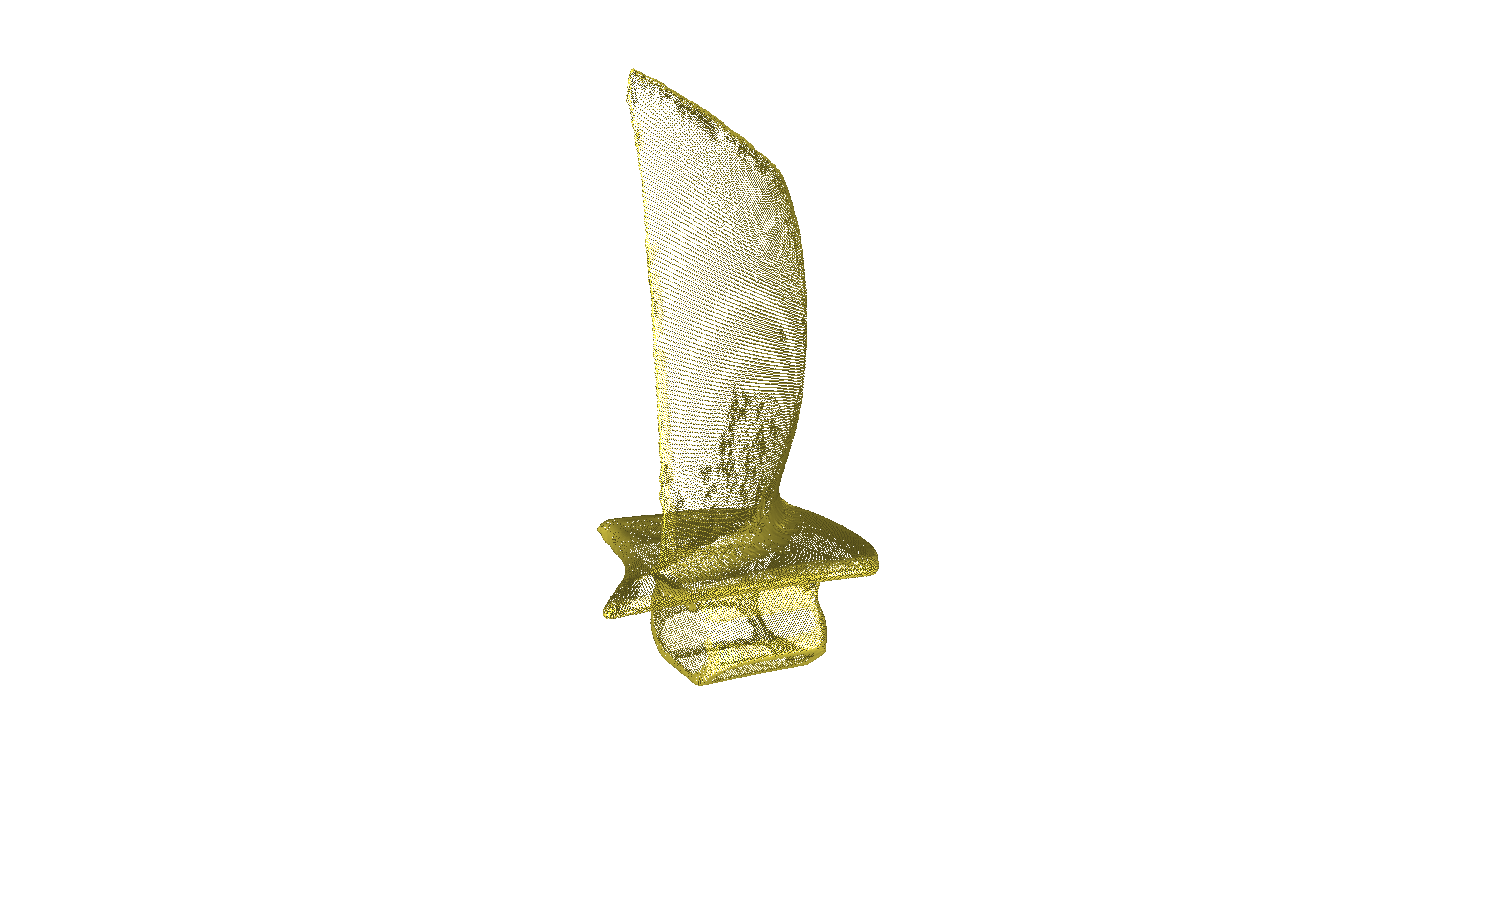
\includegraphics[width=0.8\textwidth]{scan1}
    \caption{Stage 6 Point Cloud}
    \label{fig:scan1}
\end{figure}

\section{Point Cloud Processing and CAD Model Creation}
\label{sec:cad}

To generate the CAD model from the scanned data, the point cloud was processed and imported into SolidWorks using the Xtract3D add-in. This tool facilitated working directly with the point cloud by enabling reference geometry creation and surface sculpting based on the scanned data.

Unlike traditional workflows where an STL file is imported as a surface body to optimize processing, Xtract3D allowed for direct manipulation of the point cloud without losing critical geometric information. This streamlined the modeling process, reducing the need for intermediate conversions and preserving the fidelity of the scanned data.

Using the Xtract3D slice feature, cross-sections were extracted from the point cloud, as represented in Figure~\ref{fig:slice}. This allows guiding the creation of accurate profiles and lofted surfaces that replicated the original blade geometry with high precision. By leveraging these tools, the CAD model was refined iteratively to match the scanned data while ensuring manufacturability and compatibility with further analysis.

\begin{figure}[H]
    \centering
    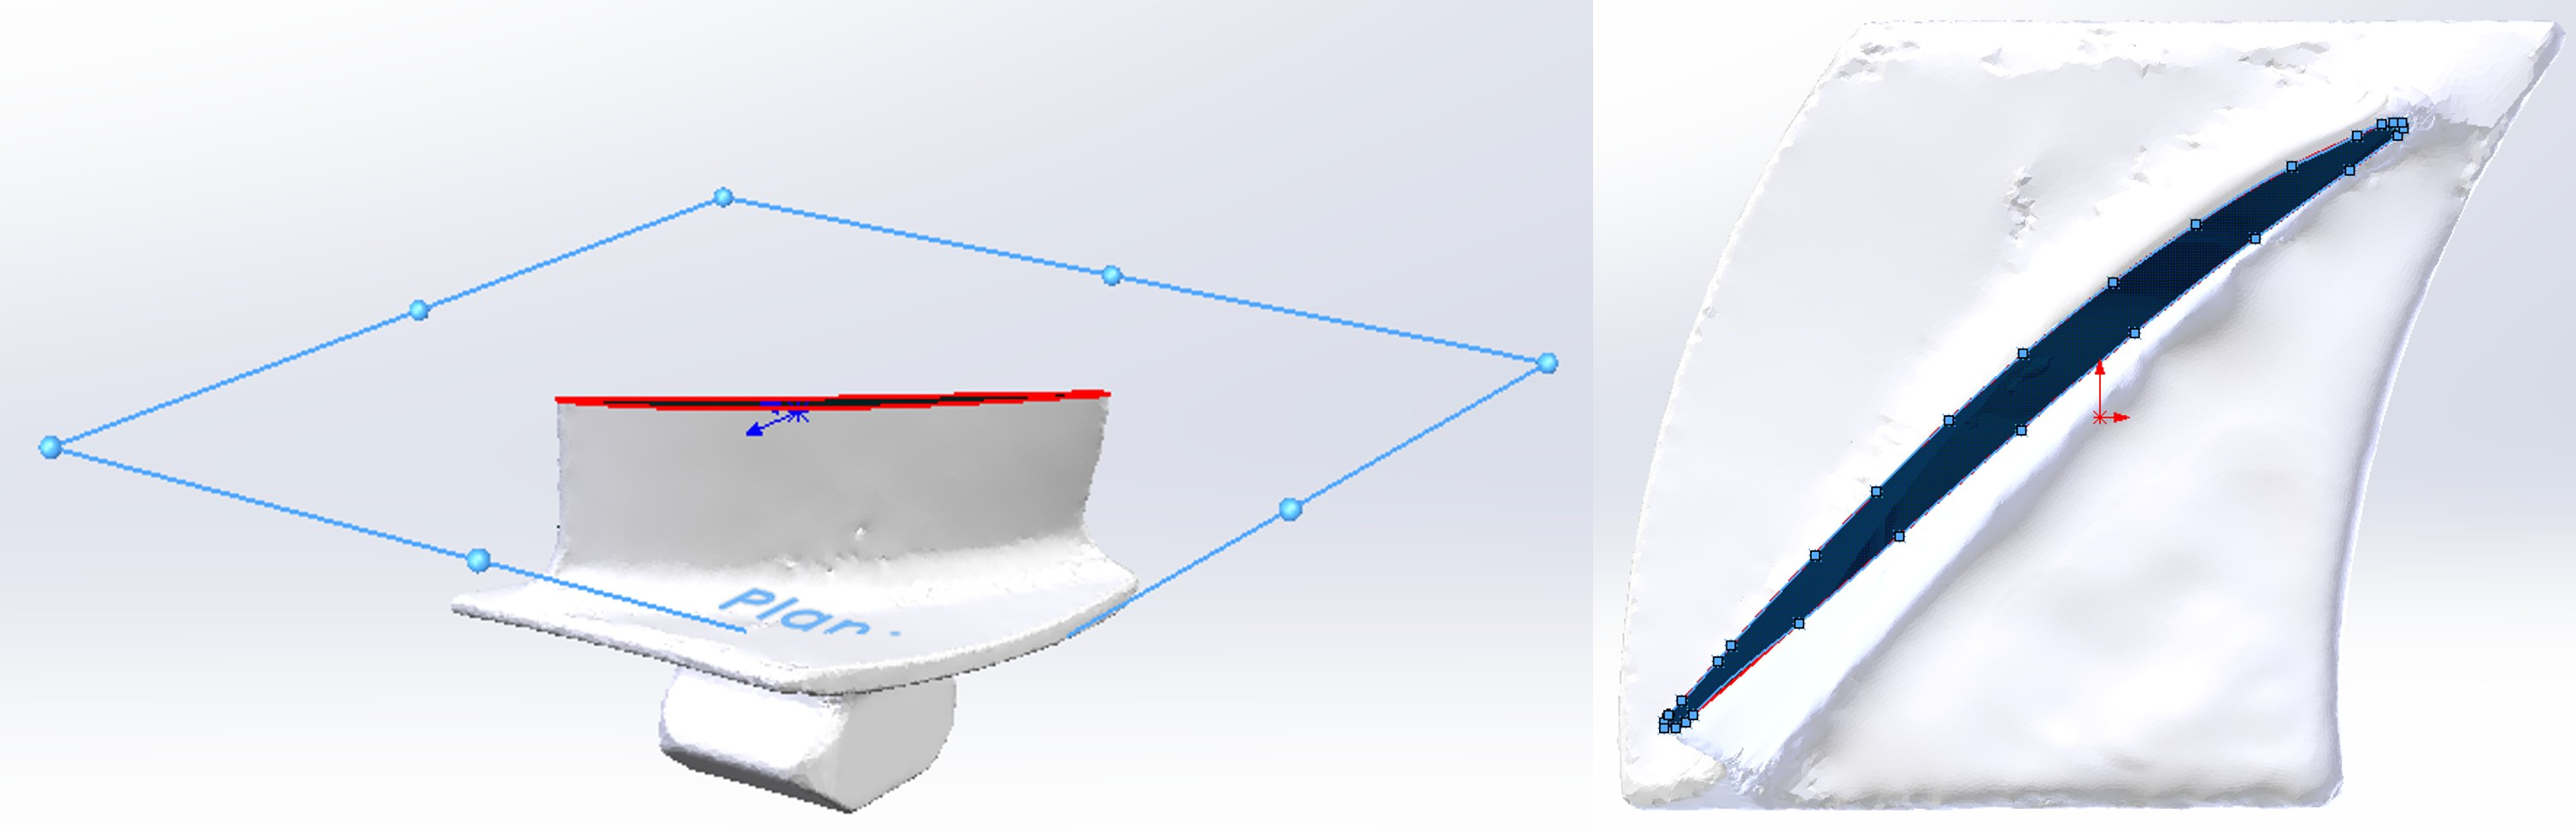
\includegraphics[width=0.8\textwidth]{slice}
    \caption{Mesh and CAD Comparison}
    \label{fig:slice}
\end{figure}

As illustrated in Figure~\ref{fig:compare.png}, this process enables the generation of an accurate CAD model from the scanned data.

\begin{figure}[H]
    \centering
    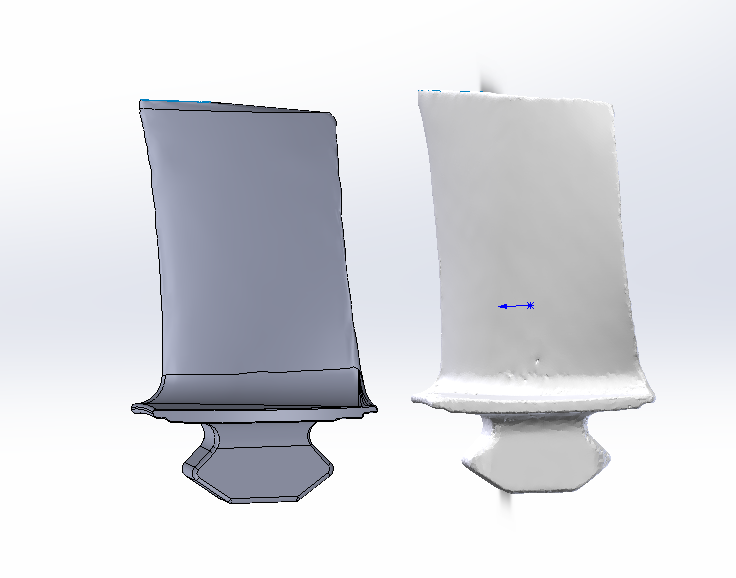
\includegraphics[width=0.5\textwidth]{compare.png}
    \caption{Mesh and CAD Comparison}
    \label{fig:compare.png}
\end{figure}

In the next section, the accuracy of the generated model will be evaluated against the scanned blade, accompanied by additional analyses, in order to ensure a parametric model accurate enough to support the development of this dissertation.
